\documentclass[../main.tex]{subfiles}
\begin{document}
    \begin{frame}
        \frametitle{1: Marker detection}
        \begin{figure}[!htb]
            \centering
            \subfloat[\small{ps3-1-a-1}]{\frame{
\includegraphics[keepaspectratio,height=0.65\textheight,width=0.45\textwidth]{ps3-1-a-1}} } \hspace{3em}
            \subfloat[\small{ps3-1-a-2}]{\frame{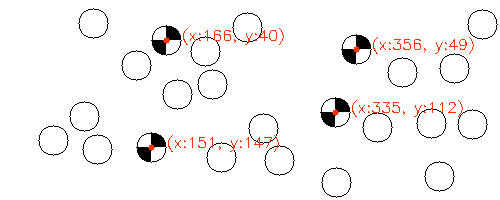
\includegraphics[keepaspectratio,height=0.65\textheight,width=0.45\textwidth]{ps3-1-a-2}}}

        \end{figure}
    \end{frame}
    
    \begin{frame}
        \frametitle{1: Marker detection (cont.)}
        \begin{figure}[!htb]
            \centering
            \frame{
\includegraphics[keepaspectratio,height=0.65\textheight,width=0.45\textwidth]{ps3-1-a-3}}
            \caption{ps3-1-a-3} 
        \end{figure}    
    \end{frame}
    
\end{document}